\section{Introduction}\label{SecIntro}

With the emergence of a new generation of trusted personal devices
(mobile phones, PDAs, \emph{etc.}), the demand for
techniques to guarantee application security has become even more
prominent. A common approach is to monitor executions with a security
automaton~\cite{Schneider99}. Upon entry or exit of a
security-critical method, the security automaton updates its internal
state. If it reaches an ``illegal'' state, the application will be
stopped and a security violation will be reported. This approach is
particularly suited for properties that are expressed as sequences of
legal method calls, such as life cycle properties, or constraints that
express how often or under which conditions a method can be called.
%
However, such a monitoring approach is not suited for all
applications, depending on their nature and use; sometimes statical
means to enforce security are necessary.

% A commonly advocated approach is to require that the application carries a
% correctness proof with it, which can be validated before installing the
% application on the device. In such a proof carrying code scenario~\cite{Necula97},
% the application provider is required to create this proof.

Security experts typically express security requirements by a collection of
security automata or temporal logic formulae. However, many program
verification tools use a Hoare logic style for the specifications
(\emph{i.e.}, pre- and postconditions).
Therefore, as a first step towards static
verification of such security properties, this paper proposes a
translation from security properties expressed as an automaton
% (or a safety temporal logic formula, which can be translated into an
% automaton~\cite{Wolper01})
into program annotations.

The translation in this paper is defined for Java programs. It is
defined in several steps. For each step we provide a correctness
proof.
\begin{inparaenum}[(\itshape i\upshape)]
\item We translate a \emph{partial automaton} to a \emph{total automaton}
that contains a special trap state to model that an error has
occurred.
% Often it is much more intuitive to specify a security property by a partial
% automaton, (this avoids cluttering up the automaton with transitions that
% \emph{``go wrong''}), while for many tools and algorithms, a complete
% automaton is easier to handle.
We show that the behaviour of a program monitored with a partial
automaton is equivalent to the behaviour of the program monitored with
the total automaton.
\item Using an extension of JML~\cite{LeavensPCCRCK05}, we generate annotations
that capture the behaviour of the total automaton. These are special
method-level set-annotations that are evaluated upon entry or exit of
a method.  We show that run-time monitoring of the program only throws
a (new) exception to signal an annotation violation if the monitor
reaches the trap state, otherwise the annotated program has the same
executions as the monitored program.
\item We inline the set-annotations from the method specification
to the method body and prove equivalence of the run-time checking behaviour.
\end{inparaenum}
All results in the paper have been established formally using
the PVS theorem prover~\cite{OwreRRSS96}. The complete formalisation
is available via \url{http://www.cs.ru.nl/~tamalet/}. To be able to
establish the correctness proof, the order in which method
specifications are evaluated is important. Further, we had to add an
explicit requirement that \texttt{finally} blocks could not override
annotation violation exceptions thrown inside \texttt{try} or
\texttt{catch} statements (see also~\cite{Huisman08}). The last
complication that we encountered was how to specify conveniently that
specification-only constructs and steps taken by the monitor did not
have any side-effects on the program state. More detailed information
about the proofs is given in Section~\ref{SecAnnotGen}.

\psfrag{s1}{\tiny{\(s_1\)}}
\psfrag{s2}{\tiny{\(s_2\)}}
\psfrag{exit(sendSMS)? true -> n := n + 1;}
{\begin{tabular}{l}
\tiny{\exit(\texttt{SendSMS})?\ttt\(\rightarrow\)}\vspace*{-.8em}\\
\tiny{\texttt{n := n + 1};}
\end{tabular}}
\psfrag{exitE(sendSMS)? true -> ;}
{\begin{tabular}{l}
\tiny{\excexit(\texttt{sendSMS})?\ttt \(\rightarrow\)}%\vspace*{-.8em}\\
\tiny{\actskip;}
\end{tabular}}
\psfrag{exit(reset)? true -> n := 0;}
{\begin{tabular}{l}
\tiny{\exit(\texttt{reset})?\ttt \(\rightarrow\)}\vspace*{-.8em} \\
\tiny{\texttt{n :=} 0;}
\end{tabular}}
\psfrag{entry(sendSMS)? n < N -> ;}
{\begin{tabular}{l}
\tiny{\entry(\texttt{sendSMS})? \texttt{n} \(<\) \texttt{N} \(\rightarrow\)} %\vspace*{-.8em} \\
\tiny{\actskip;}
\end{tabular}}
\begin{floatingfigure}{6cm}
\begin{center}
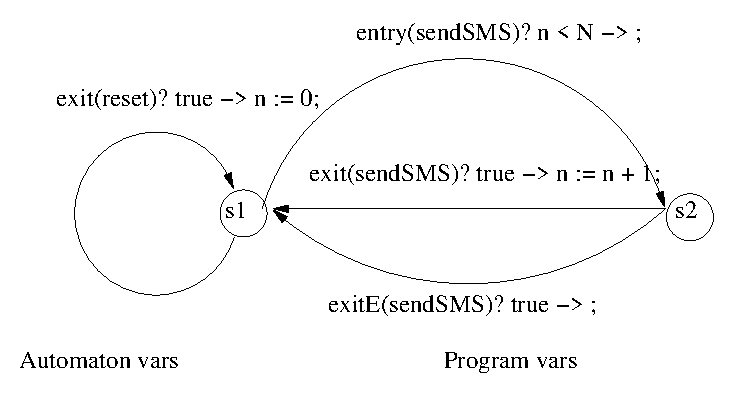
\epsfig{file=limited_sms.eps, width=5.5cm}
\end{center}
\caption{Example Security Automaton}\label{FigExample}
\end{floatingfigure}
Throughout this paper, we use the \emph{limited SMS} example property of
Figure~\ref{FigExample} (where \(\epsilon\) denotes a skip) to
illustrate the different translations: the method \texttt{sendSMS} can
be called and terminate successfully at most \(N\) times in between
calls to a \texttt{reset} method. Notice that the counter is not
increased if \texttt{sendSMS} terminates with an uncaught exception
(labelled \excexit{(\texttt{sendSMS})}), and that \texttt{reset}
should not be called from within \texttt{sendSMS}.  Even though very
basic, this example is representative of a wide range of important
resource-related security properties.

The rest of this paper is organised as follows.  Section~\ref{SecMVA}
formalises the automaton format and defines completion. Next,
Section~\ref{SecProgram} defines the semantics of monitored and
annotated programs. Section~\ref{SecAnnotGen} defines the
translation and proves correctness. Sections~\ref{SecRelated}
and~\ref{SecConcl} discuss related and future work and conclusions.
